\documentclass[notheorems, handout]{beamer}

\usetheme{warsaw}
\setbeamertemplate{page number in head/foot}[totalframenumber]
\setbeamertemplate{headline}{}
\setbeamertemplate{navigation symbols}{}
\usefonttheme[onlymath]{serif}

\usepackage[utf8]{inputenc}
\usepackage[T2A]{fontenc}
\usepackage[russian]{babel}

\usepackage{graphicx,subcaption,ragged2e}
\usepackage{tikz}
\usepackage{bm}

\setbeamercolor{bluetext_color}{fg=blue}
\newcommand{\bluetext}[1]{{\usebeamercolor[fg]{bluetext_color}#1}}

\usetikzlibrary{shapes.geometric, arrows}
\tikzstyle{arrow} = [thick,->,>=stealth]

\title[Выделение сигнала на основе MC-SSA]{Выделение сигнала на основе критерия Monte Carlo SSA}

\author[Потешкин\,Е.\,П., Голяндина\,Н.\,Э.]{\underline{Потешкин Егор Павлович}, Голяндина Нина Эдуардовна}

\institute[Санкт-Петербургский Государственный Университет]{%
	\small
	Санкт-Петербургский государственный университет\\
	Кафедра статистического моделирования}

\date{\\Мат-Мех. Наука 2025\\30 апреля 2025, Санкт-Петербург}

\subject{Talks}	

%new calligraphic font for subspaces 
\usepackage{euscript}
\newcommand{\cA}{\EuScript{A}}
\newcommand{\cB}{\EuScript{B}}
\newcommand{\cC}{\EuScript{C}}
\newcommand{\cD}{\EuScript{D}}
\newcommand{\cE}{\EuScript{E}}
\newcommand{\cF}{\EuScript{F}}
\newcommand{\cG}{\EuScript{G}}
\newcommand{\cH}{\EuScript{H}}
\newcommand{\cI}{\EuScript{I}}
\newcommand{\cJ}{\EuScript{J}}
\newcommand{\cK}{\EuScript{K}}
\newcommand{\cL}{\EuScript{L}}
\newcommand{\cM}{\EuScript{M}}
\newcommand{\cN}{\EuScript{N}}
\newcommand{\cO}{\EuScript{O}}
\newcommand{\cP}{\EuScript{P}}
\newcommand{\cQ}{\EuScript{Q}}
\newcommand{\cR}{\EuScript{R}}
\newcommand{\cS}{\EuScript{S}}
\newcommand{\cT}{\EuScript{T}}
\newcommand{\cU}{\EuScript{U}}
\newcommand{\cV}{\EuScript{V}}
\newcommand{\cW}{\EuScript{W}}
\newcommand{\cX}{\EuScript{X}}
\newcommand{\cY}{\EuScript{Y}}
\newcommand{\cZ}{\EuScript{Z}}

%font for text indices like transposition X^\mathrm{T}
\newcommand{\rmA}{\mathrm{A}}
\newcommand{\rmB}{\mathrm{B}}
\newcommand{\rmC}{\mathrm{C}}
\newcommand{\rmD}{\mathrm{D}}
\newcommand{\rmE}{\mathrm{E}}
\newcommand{\rmF}{\mathrm{F}}
\newcommand{\rmG}{\mathrm{G}}
\newcommand{\rmH}{\mathrm{H}}
\newcommand{\rmI}{\mathrm{I}}
\newcommand{\rmJ}{\mathrm{J}}
\newcommand{\rmK}{\mathrm{K}}
\newcommand{\rmL}{\mathrm{L}}
\newcommand{\rmM}{\mathrm{M}}
\newcommand{\rmN}{\mathrm{N}}
\newcommand{\rmO}{\mathrm{O}}
\newcommand{\rmP}{\mathrm{P}}
\newcommand{\rmQ}{\mathrm{Q}}
\newcommand{\rmR}{\mathrm{R}}
\newcommand{\rmS}{\mathrm{S}}
\newcommand{\rmT}{\mathrm{T}}
\newcommand{\rmU}{\mathrm{U}}
\newcommand{\rmV}{\mathrm{V}}
\newcommand{\rmW}{\mathrm{W}}
\newcommand{\rmX}{\mathrm{X}}
\newcommand{\rmY}{\mathrm{Y}}
\newcommand{\rmZ}{\mathrm{Z}}

%tt font for time series
\newcommand{\tA}{\mathsf{A}}
\newcommand{\tB}{\mathsf{B}}
\newcommand{\tC}{\mathsf{C}}
\newcommand{\tD}{\mathsf{D}}
\newcommand{\tE}{\mathsf{E}}
\newcommand{\tF}{\mathsf{F}}
\newcommand{\tG}{\mathsf{G}}
\newcommand{\tH}{\mathsf{H}}
\newcommand{\tI}{\mathsf{I}}
\newcommand{\tJ}{\mathsf{J}}
\newcommand{\tK}{\mathsf{K}}
\newcommand{\tL}{\mathsf{L}}
\newcommand{\tM}{\mathsf{M}}
\newcommand{\tN}{\mathsf{N}}
\newcommand{\tO}{\mathsf{O}}
\newcommand{\tP}{\mathsf{P}}
\newcommand{\tQ}{\mathsf{Q}}
\newcommand{\tR}{\mathsf{R}}
\newcommand{\tS}{\mathsf{S}}
\newcommand{\tT}{\mathsf{T}}
\newcommand{\tU}{\mathsf{U}}
\newcommand{\tV}{\mathsf{V}}
\newcommand{\tW}{\mathsf{W}}
\newcommand{\tX}{\mathsf{X}}
\newcommand{\tY}{\mathsf{Y}}
\newcommand{\tZ}{\mathsf{Z}}

%bf font for matrices
\newcommand{\bfA}{\mathbf{A}}
\newcommand{\bfB}{\mathbf{B}}
\newcommand{\bfC}{\mathbf{C}}
\newcommand{\bfD}{\mathbf{D}}
\newcommand{\bfE}{\mathbf{E}}
\newcommand{\bfF}{\mathbf{F}}
\newcommand{\bfG}{\mathbf{G}}
\newcommand{\bfH}{\mathbf{H}}
\newcommand{\bfI}{\mathbf{I}}
\newcommand{\bfJ}{\mathbf{J}}
\newcommand{\bfK}{\mathbf{K}}
\newcommand{\bfL}{\mathbf{L}}
\newcommand{\bfM}{\mathbf{M}}
\newcommand{\bfN}{\mathbf{N}}
\newcommand{\bfO}{\mathbf{O}}
\newcommand{\bfP}{\mathbf{P}}
\newcommand{\bfQ}{\mathbf{Q}}
\newcommand{\bfR}{\mathbf{R}}
\newcommand{\bfS}{\mathbf{S}}
\newcommand{\bfT}{\mathbf{T}}
\newcommand{\bfU}{\mathbf{U}}
\newcommand{\bfV}{\mathbf{V}}
\newcommand{\bfW}{\mathbf{W}}
\newcommand{\bfX}{\mathbf{X}}
\newcommand{\bfY}{\mathbf{Y}}
\newcommand{\bfZ}{\mathbf{Z}}

%bb font for standard spaces and expectation
\newcommand{\bbA}{\mathbb{A}}
\newcommand{\bbB}{\mathbb{B}}
\newcommand{\bbC}{\mathbb{C}}
\newcommand{\bbD}{\mathbb{D}}
\newcommand{\bbE}{\mathbb{E}}
\newcommand{\bbF}{\mathbb{F}}
\newcommand{\bbG}{\mathbb{G}}
\newcommand{\bbH}{\mathbb{H}}
\newcommand{\bbI}{\mathbb{I}}
\newcommand{\bbJ}{\mathbb{J}}
\newcommand{\bbK}{\mathbb{K}}
\newcommand{\bbL}{\mathbb{L}}
\newcommand{\bbM}{\mathbb{M}}
\newcommand{\bbN}{\mathbb{N}}
\newcommand{\bbO}{\mathbb{O}}
\newcommand{\bbP}{\mathbb{P}}
\newcommand{\bbQ}{\mathbb{Q}}
\newcommand{\bbR}{\mathbb{R}}
\newcommand{\bbS}{\mathbb{S}}
\newcommand{\bbT}{\mathbb{T}}
\newcommand{\bbU}{\mathbb{U}}
\newcommand{\bbV}{\mathbb{V}}
\newcommand{\bbW}{\mathbb{W}}
\newcommand{\bbX}{\mathbb{X}}
\newcommand{\bbY}{\mathbb{Y}}
\newcommand{\bbZ}{\mathbb{Z}}

%got font for any case
\newcommand{\gA}{\mathfrak{A}}
\newcommand{\gB}{\mathfrak{B}}
\newcommand{\gC}{\mathfrak{C}}
\newcommand{\gD}{\mathfrak{D}}
\newcommand{\gE}{\mathfrak{E}}
\newcommand{\gF}{\mathfrak{F}}
\newcommand{\gG}{\mathfrak{G}}
\newcommand{\gH}{\mathfrak{H}}
\newcommand{\gI}{\mathfrak{I}}
\newcommand{\gJ}{\mathfrak{J}}
\newcommand{\gK}{\mathfrak{K}}
\newcommand{\gL}{\mathfrak{L}}
\newcommand{\gM}{\mathfrak{M}}
\newcommand{\gN}{\mathfrak{N}}
\newcommand{\gO}{\mathfrak{O}}
\newcommand{\gP}{\mathfrak{P}}
\newcommand{\gQ}{\mathfrak{Q}}
\newcommand{\gR}{\mathfrak{R}}
\newcommand{\gS}{\mathfrak{S}}
\newcommand{\gT}{\mathfrak{T}}
\newcommand{\gU}{\mathfrak{U}}
\newcommand{\gV}{\mathfrak{V}}
\newcommand{\gW}{\mathfrak{W}}
\newcommand{\gX}{\mathfrak{X}}
\newcommand{\gY}{\mathfrak{Y}}
\newcommand{\gZ}{\mathfrak{Z}}

%old calligraphic font
\newcommand{\calA}{\mathcal{A}}
\newcommand{\calB}{\mathcal{B}}
\newcommand{\calC}{\mathcal{C}}
\newcommand{\calD}{\mathcal{D}}
\newcommand{\calE}{\mathcal{E}}
\newcommand{\calF}{\mathcal{F}}
\newcommand{\calG}{\mathcal{G}}
\newcommand{\calH}{\mathcal{H}}
\newcommand{\calI}{\mathcal{I}}
\newcommand{\calJ}{\mathcal{J}}
\newcommand{\calK}{\mathcal{K}}
\newcommand{\calL}{\mathcal{L}}
\newcommand{\calM}{\mathcal{M}}
\newcommand{\calN}{\mathcal{N}}
\newcommand{\calO}{\mathcal{O}}
\newcommand{\calP}{\mathcal{P}}
\newcommand{\calQ}{\mathcal{Q}}
\newcommand{\calR}{\mathcal{R}}
\newcommand{\calS}{\mathcal{S}}
\newcommand{\calT}{\mathcal{T}}
\newcommand{\calU}{\mathcal{U}}
\newcommand{\calV}{\mathcal{V}}
\newcommand{\calW}{\mathcal{W}}
\newcommand{\calX}{\mathcal{X}}
\newcommand{\calY}{\mathcal{Y}}
\newcommand{\calZ}{\mathcal{Z}}


\begin{document}
\begin{frame}[plain]
	\titlepage
	\note{Научный руководитель  д.ф.-м.н., профессор Голяндина\,Н.\,Э.,\\
		кафедра статистического моделирования}
\end{frame}

\begin{frame}{Есть ли сигнал?}
	\begin{figure}
		\centering
		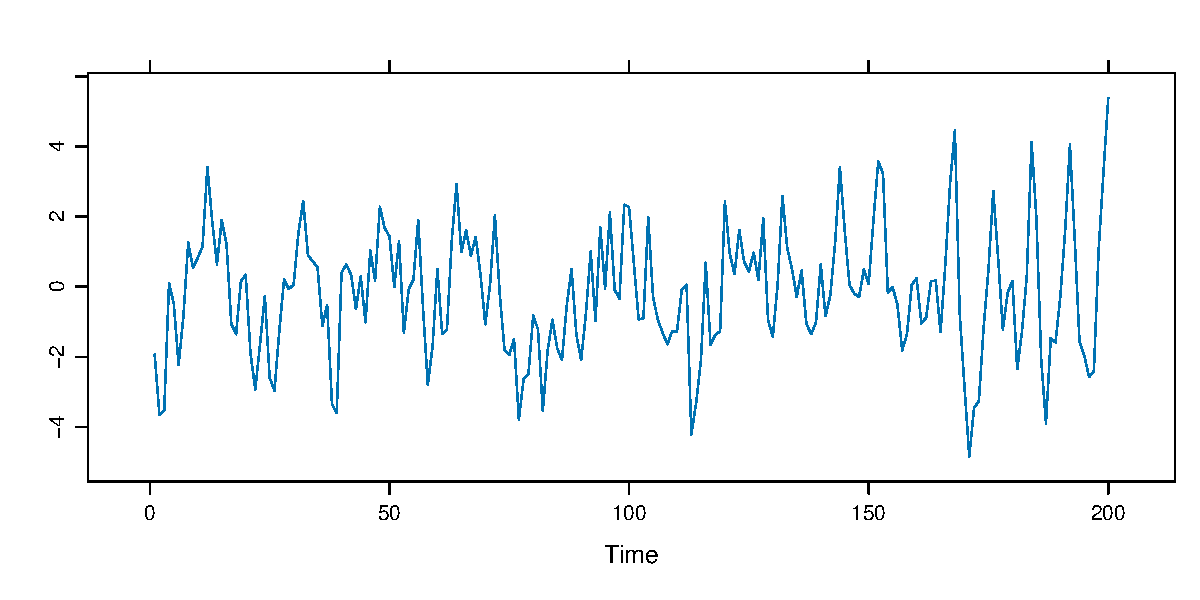
\includegraphics[width=\textwidth]{img/noise_ts.pdf}
	\end{figure}
	\bluetext{Вопрос}: это чистый шум или там есть сигнал?
\end{frame}

\begin{frame}{Постановка задачи}
	$\tX=(x_1,\ldots,x_N)$, $x_i\in \mathbb{R}$~--- временной ряд.\medskip

	\bluetext{Дано}: $\tX=\tT + \tH + \tR$, где $\tT$~--- тренд, $\tH$~--- периодическая компонента и $\tR$~--- шум.\medskip

	\bluetext{Проблемы}:
	\begin{enumerate}
		\item Как проверить наличие сигнала $\tS=\tT + \tH$?
		\item Как выделить сигнал $\tS$, если он есть?\medskip
	\end{enumerate}

	\bluetext{Методы}:
	\begin{enumerate}
		\item Monte-Carlo SSA (MC-SSA)~[Allen and Smith, 1996] проверяет $H_0:\tS=0$.
		\item Singular spectrum analysis\linebreak(SSA)~[Golyandina, Nekrutkin and Zhigljavsky, 2001].\medskip
	\end{enumerate}
	\bluetext{Задача}: реализовать алгоритм автоматического выделения сигнала на основе MC-SSA.
\end{frame}

\begin{frame}{Обозначения и известные результаты: оператор вложения и ганкелизации}
	$\tX=(x_1,\ldots,x_N)$. Зафиксируем $L$ ($1<L<N$).\medskip

	\emph{Оператор вложения} $\cT_\text{SSA}$:
	\begin{equation*}
		\cT_{\text{SSA}}(\tX)=\bfX=\begin{pmatrix}
			x_1    & x_2     & \cdots & x_K     \\
			x_2    & x_3     & \cdots & x_{K+1} \\
			\vdots & \vdots  & \ddots & \vdots  \\
			x_L    & x_{L+1} & \cdots & x_N
		\end{pmatrix},
	\end{equation*}
	где $K=N-L+1$.\medskip

	\emph{Оператор ганкелизации} $\cH$~--- усреднение матрицы по побочным диагоналям.
\end{frame}

\begin{frame}{Обозначения и известные результаты: алгоритм SSA}
	\bluetext{Входные данные}: временной ряд $\tX=(x_1,\ldots,x_N)$.\\

	\bluetext{Параметры}: длина окна $L$, набор индексов $I\subset\{1,\ldots,d\}$. \\

	\bluetext{Выходные данные}: оценка сигнала.\medskip

	\begin{figure}
		\scalebox{0.5}{
			\begin{tikzpicture}[node distance=2cm]
				\node[draw, align=center, minimum width=8.5cm, minimum height=3.25cm](1){{\LARGE\textbf{Входные данные}: $\tX$}~---\\\LARGE временной ряд};
				\node[draw, align=center, minimum width=8.5cm, minimum height=3.25cm, below of=1, yshift=-2cm](2){{\LARGE Траекторная матрица}\\ \LARGE $\bf{X}=\cT_{\text{SSA}}(\tX)$};
				\node[draw, align=center, minimum width=8.5cm, minimum height=3.25cm, right of=2, xshift=10cm](3){\LARGE Сумма матриц\\ \LARGE единичного ранга\\ \LARGE$\bfX=\sum\limits_{j=1}^d\bfX_j$};
				\node[draw, align=center, minimum width=8.5cm, minimum height=3.25cm, below of=3, yshift=-2cm](4){\LARGE Группировка матриц,\\ \LARGE соответствующих сигналу\\ \LARGE$\bfX=\bfX_{I}+(\bfX-\bfX_{I})$\\\LARGE$\bfX_{I}=\sum\limits_{i\in I}\bfX_i$};
				\node[draw, align=center, minimum width=8.5cm, minimum height=3.25cm, below of=2, yshift=-2cm](5){\LARGE\textbf{Результат}: SSA разложение\\\LARGE$\tX=\widetilde\tS+\widetilde{\tR}$\\\LARGE$\widetilde\tS=\cT_\text{SSA}^{-1}\circ\cH(\bfX_{I})$};

				\draw[arrow](1)--node[anchor=west]{\large1. Вложение}(2);
				\draw[arrow](2)--node[anchor=south]{\large2. Разложение}(3);
				\draw[arrow](3)--node[anchor=west]{\large3. Группировка}(4);
				\draw[arrow](4)--node[anchor=south]{\large4. Восстановление}(5);
			\end{tikzpicture}}
	\end{figure}
\end{frame}

\begin{frame}{Пример: применение SSA}
	\begin{figure}
		\centering
		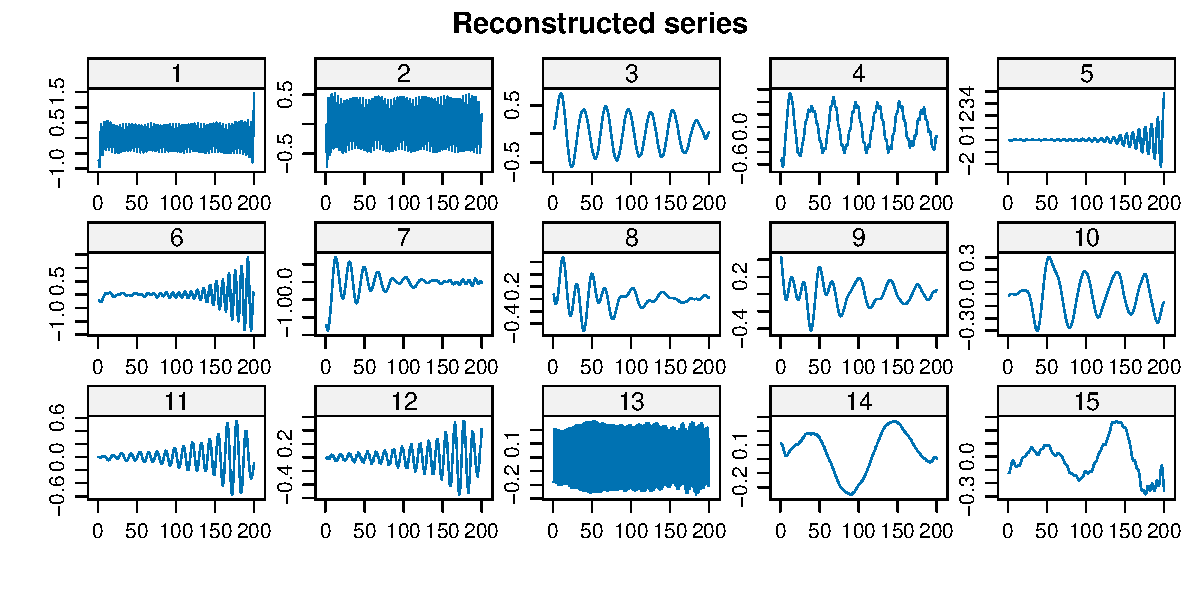
\includegraphics[width=\textwidth]{img/reconstructed_ts.pdf}
		\caption{Элементарные восстановленные компоненты ($L=100$)}
	\end{figure}
	Компоненты, соответствующие сигналу: $1$, $2$, $5$, $6$ и $13$.
\end{frame}

\begin{frame}{Обозначения и известные результаты: Monte-Carlo SSA}
	\bluetext{Входные данные}: $\tX=\tS+\tR$, где $\tS$~--- сигнал, $\tR$~--- реализация стационарного процесса $\bm\xi$ с нулевым средним и со спектральной плотностью $f_{\bm\theta}$.\medskip

	\bluetext{Параметры}: длина окна $L$, $W_1,\ldots, W_M\in \mathbb R^L$~--- нормированные векторы, соответствующие определенным частотам.\medskip

	\bluetext{Статистика критерия}: величины
	$$
	\widehat p_k = \left\|\bfX^\rmT W_k\right\|^2.
	$$

	Распределение $\widehat p_k$ при верной $H_0$, вообще говоря, неизвестно~--- оно оценивается с помощью метода Monte Carlo.\medskip

	Multiple MC-SSA~[Golyandina, 2023]: модификация MC-SSA с поправкой на множественные сравнения.\medskip

	В качестве $W_k$ рассматриваются косинусы с равностоящими частотами $\omega_k=k/(2L)$, $k=1,\ldots, L$.
\end{frame}

\begin{frame}{Обозначения и известные результаты: оценка параметров шума}
	Параметры шума $\bm\theta$, вообще говоря, неизвестны, поэтому их нужно оценивать.\medskip

	Получить оценки параметров можно, максимизируя правдоподобие Whittle~[Whittle, 1953]:
	$$
	\ell_W(\bm\theta)=-\frac{1}{m}\sum_{j=1}^m\left(\ln f_{\bm\theta}(\omega_j)+\frac{I_N(\omega_j)}{f_{\bm\theta}(\omega_j)}\right),
	$$
	где $m=\lfloor (N-1)/2\rfloor$, $f_{\bm\theta}$~--- спектральная плотность $\bm\xi$, $I_N$~--- периодограмма исходного ряда, $\omega_j=j/N$.\medskip

	Оценивать параметры можно по части спектра: пусть $J=\{j_1, \ldots, j_p\}$~--- индексы частот, которые мы не хотим учитывать при оценке параметров. Тогда при вычислении $\ell_W(\bm\theta)$ рассматриваются только индексы $j\not\in J$.
\end{frame}

\begin{frame}{Пример: применение Monte Carlo SSA}
	$\tX=\tS+\boldsymbol{\xi}$, где $\boldsymbol{\xi}$~--- красный шум с параметрами $\phi=0.7$ и $\sigma^2=1$, $N=200$,
	$$
	s_n=0.075\,e^{0.02n}\cos(2\pi n / 8) + 2\cos(2\pi n / 4) + 0.2\cdot (-1)^n.
	$$
	\begin{figure}
		\centering
		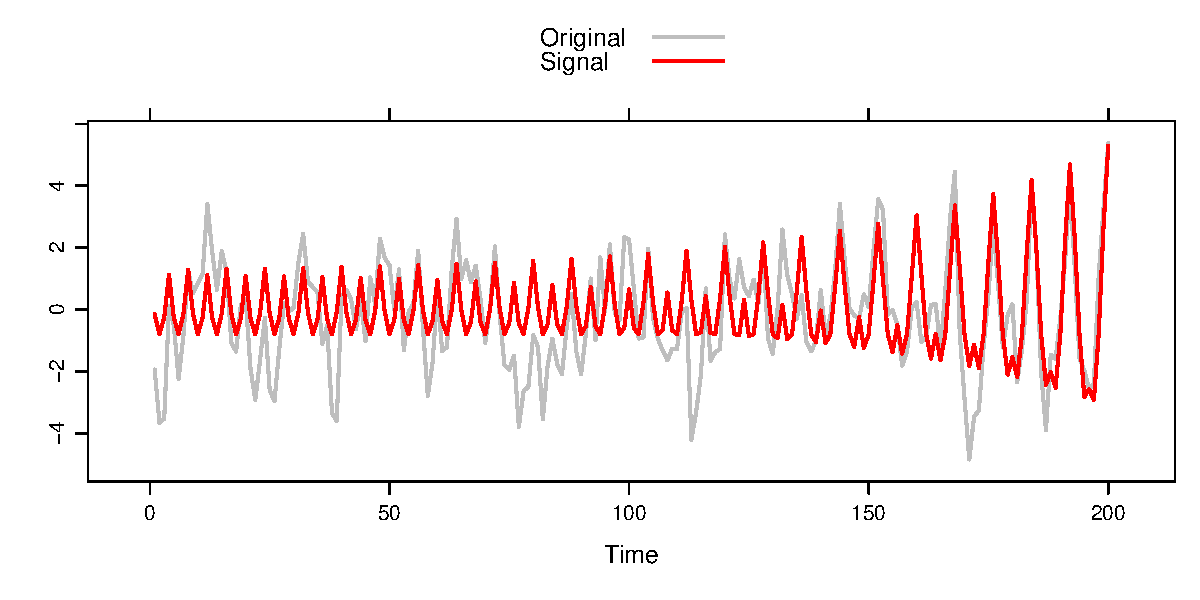
\includegraphics[width=\textwidth]{img/noise_ts_signal.pdf}
	\end{figure}
\end{frame}

\begin{frame}{Пример: применение Monte Carlo SSA}
	\begin{figure}
		\centering
		\minipage{0.5\textwidth}
			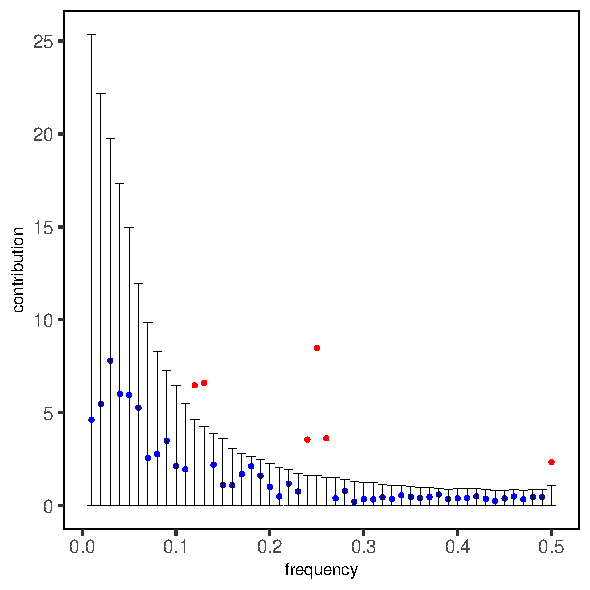
\includegraphics[width=0.9\textwidth]{img/mcssa_real.pdf}
			\caption{Истинная модель шума}
		\endminipage\hfill
		\minipage{0.5\textwidth}
			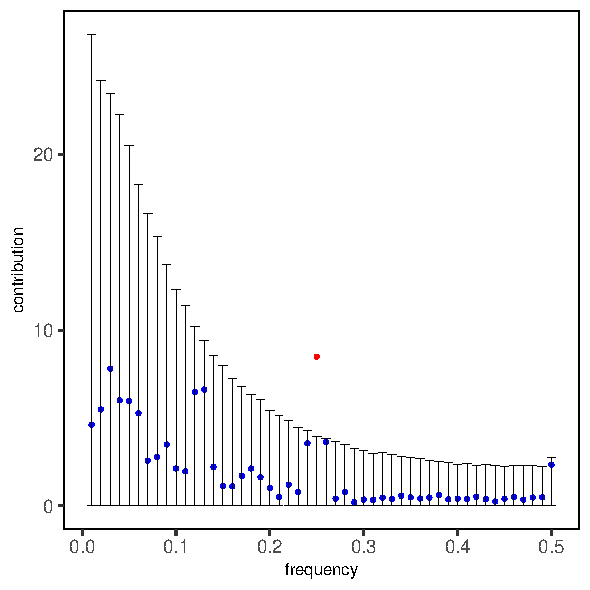
\includegraphics[width=0.9\textwidth]{img/mcssa_estimated.pdf}
			\caption{Оцененная модель шума}
		\endminipage
	\end{figure}
	\textcolor{red}{Проблема}: при оценивании параметров обнаруживаются не все частоты.

	\bluetext{Решение}: итеративно применять критерий после выделения одной гармоники, пока гипотеза $H_0:\tS=0$ отвергается.
\end{frame}

\begin{frame}{Обозначения и известные результаты: автоматическая группировка в SSA}
	Для ряда $\tX$ длины $N$ и $0\leqslant\omega_1\leqslant\omega_2\leqslant0.5$ определим меру
	$$
	T(\tX; \omega_1,\omega_2)=\frac{1}{\|\tX\|^2}\sum_{k:\omega_1\leqslant k / N \leqslant \omega_2}I_N(k / N),
	$$
	где $I_N$~--- периодограмма $\tX$. \medskip
	
	Величину $T(\tX; \omega_1, \omega_2)$ можно рассматривать как долю вклада частот, содержащегося в интервале $[\omega_1, \omega_2]$.\bigskip

	Пусть $\omega^\star$~--- значимая частота. Тогда $[\omega_1, \omega_2]=[\omega^\star-\delta, \omega^\star + \delta]$.
\end{frame}

\begin{frame}{Алгоритм autoMCSSA}
	\begin{figure}
		\centering
		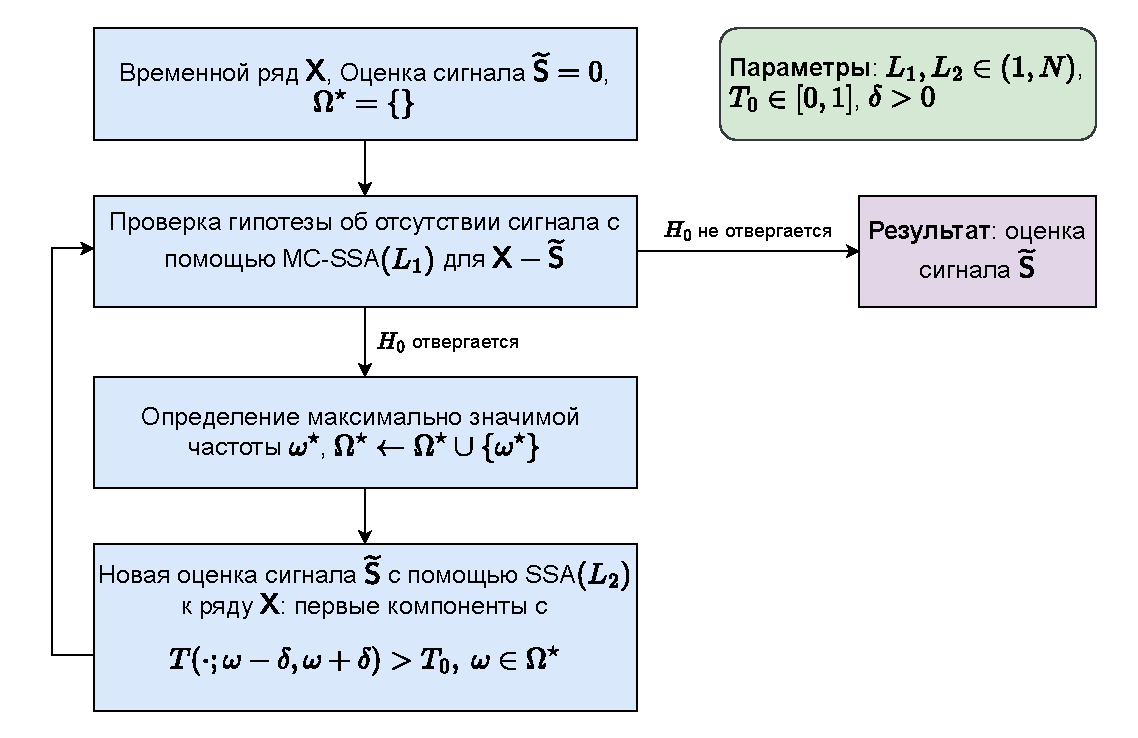
\includegraphics[width=\textwidth]{img/auto_mcssa_alg.pdf}
	\end{figure}
\end{frame}

\begin{frame}{Пример: применение autoMCSSA}
	$\tX=\tS+\boldsymbol{\xi}$, где $\boldsymbol{\xi}$~--- красный шум с параметрами $\phi=0.7$ и $\sigma^2=1$, $N=200$,
	$$
	s_n=0.075\,e^{0.02n}\cos(2\pi n / 8) + 2\cos(2\pi n / 4) + 0.2\cdot (-1)^n.
	$$\vspace{-2.5em}
	\begin{figure}
		\centering
		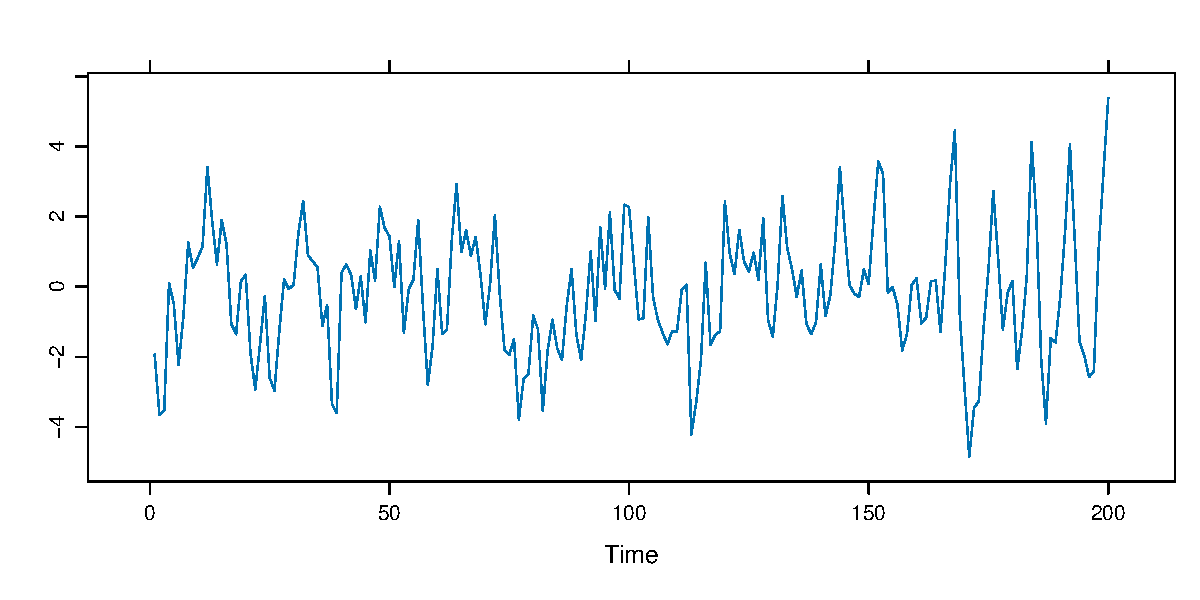
\includegraphics[width=\textwidth]{img/noise_ts.pdf}
	\end{figure}
\end{frame}

\begin{frame}{Пример: применение autoMCSSA}
	\begin{figure}
		\centering
		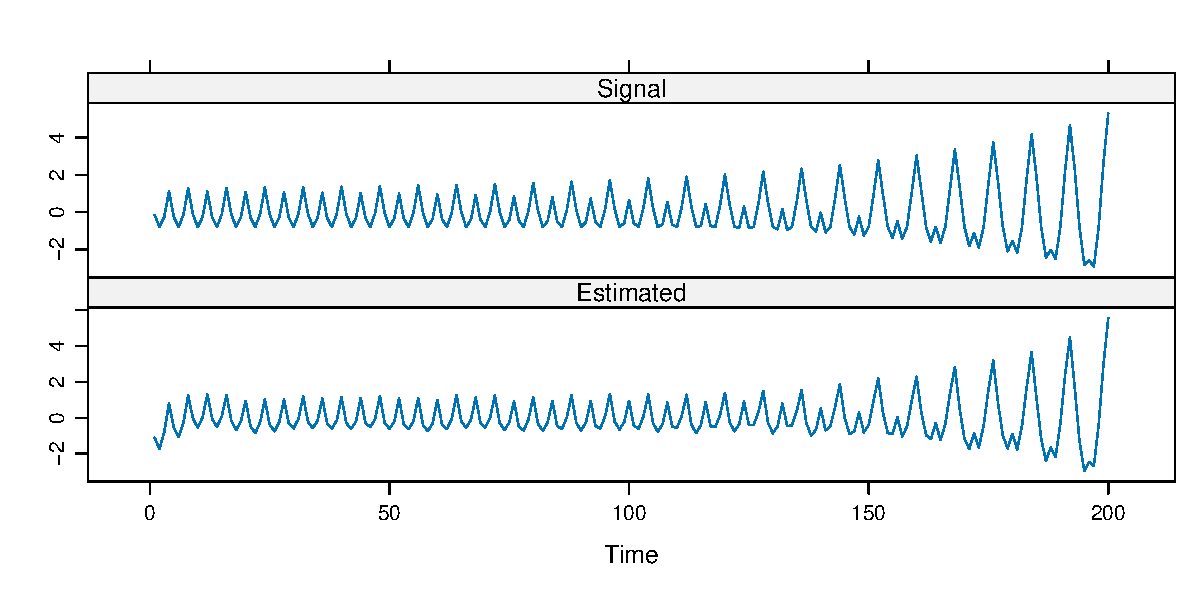
\includegraphics[width=\textwidth]{img/auto_mcssa_result.pdf}
	\end{figure}
	Параметры: $L_1=50$, $L_2=100$, $\delta=1/80$, $T_0=0.5$.\medskip

	Метод autoMCSSA правильно идентифицировал значимые компоненты (1, 2, 5, 6 и 13).
\end{frame}

\begin{frame}{Численное сравнение с autoSSA}
	Сравним метод autoMCSSA с методом autoSSA~[Дудник, 2025].\medskip

	Рассмотрим временной ряд $\tX = \tS + \bm\xi$ длины $N=100$, где
	$$
	s_n=0.2e^{0.05 n}\cos(2\pi n/4) + 2\cos(2\pi n / 3) + (-1)^n,
	$$
	$\bm\xi$~--- красный шум с параметрами $\phi\in\{0, 0.5\}$, $\sigma^2=1$. Для autoMCSSA были выбраны следующие параметры:\smallskip
	\begin{itemize}
		\item Длины окна $L_1=20$ и $L_2=50$;\smallskip
		\item Радиус промежутка для вычисления меры $T$ $\delta = 1 / 80$;\smallskip
		\item Порог для меры $T$ $T_0=0.5$;\smallskip
		\item Максимальное количество итераций: $10$.
	\end{itemize}
\end{frame}

\begin{frame}{Численное сравнение с autoSSA}
	\begin{table}[h]
		\centering
		\caption{MSE выделения сигнала ($\phi=0$)}
		\begin{tabular}{|r|r|r|}
			\hline
			& Mean MSE & Median MSE \\ 
			\hline
			autoMCSSA & 0.15196 & 0.13921 \\ 
			\hline
			autoSSA & 0.14872 & 0.14003 \\ 
			\hline
		\end{tabular}
	\end{table}
	\begin{table}[h]
		\centering
		\caption{MSE выделения сигнала ($\phi=0.5$)}
		\begin{tabular}{|r|r|r|}
			\hline
			& Mean MSE & Median MSE \\ 
			\hline
			autoMCSSA & 0.11563 & 0.09038 \\ 
			\hline
			autoSSA & 0.09341 & 0.08795 \\ 
			\hline
		\end{tabular}
	\end{table}
\end{frame}

\begin{frame}{Итоги}
	\begin{enumerate}
		\item Был реализован метод autoMCSSA, позволяющий автоматически выделить значимый сигнал, а также модификация метода Whittle по части спектра.\medskip
		\item Получено, что autoMCSSA позволяет выделять сигнал, компоненты которого в SSA необязательно доминируют.\medskip
		\item При сравнении с autoSSA метод autoMCSSA показал сравнимый результат.\medskip
		\item Необходимо сформулировать подход к выбору параметров autoMCSSA.
	\end{enumerate}
\end{frame}
\end{document}